\documentclass[a4paper,12pt]{article}

%%% Работа с русским языком % для pdfLatex
\usepackage{cmap}					% поиск в~PDF
\usepackage{mathtext} 				% русские буквы в~фомулах
\usepackage[T2A]{fontenc}			% кодировка
\usepackage[utf8]{inputenc}			% кодировка исходного текста
\usepackage[english,russian]{babel}	% локализация и переносы
\usepackage{indentfirst} 			% отступ 1 абзаца

%%% Работа с русским языком % для XeLatex
%\usepackage[english,russian]{babel}   %% загружает пакет многоязыковой вёрстки
%\usepackage{fontspec}      %% подготавливает загрузку шрифтов Open Type, True Type и др.
%\defaultfontfeatures{Ligatures={TeX},Renderer=Basic}  %% свойства шрифтов по умолчанию
%\setmainfont[Ligatures={TeX,Historic}]{Times New Roman} %% задаёт основной шрифт документа
%\setsansfont{Comic Sans MS}                    %% задаёт шрифт без засечек
%\setmonofont{Courier New}
%\usepackage{indentfirst}
%\frenchspacing

%%% Дополнительная работа с математикой
\usepackage{amsfonts,amssymb,amsthm,mathtools}
\usepackage{amsmath}
\usepackage{icomma} % "Умная" запятая: $0,2$~--- число, $0, 2$~--- перечисление
\usepackage{upgreek}

%%% Страница
\usepackage{extsizes} % Возможность сделать 14-й шрифт

%% Шрифты
\usepackage{euscript}	 % Шрифт Евклид
\usepackage{mathrsfs} % Красивый матшрифт

%% Свои команды
\DeclareMathOperator{\sgn}{\mathop{sgn}} % создание новой конанды \sgn (типо как \sin)
\usepackage{csquotes} % ещё одна штука для цитат
\newcommand{\pd}[2]{\ensuremath{\cfrac{\partial #1}{\partial #2}}} % частная производная
\newcommand{\abs}[1]{\ensuremath{\left|#1\right|}} % модуль
\renewcommand{\phi}{\ensuremath{\varphi}} % греческая фи
\newcommand{\pogk}[1]{\!\left(\cfrac{\sigma_{#1}}{#1}\right)^{\!\!\!2}\!}

% Ссылки
\usepackage{color} % подключить пакет color
% выбрать цвета
\definecolor{BlueGreen}{RGB}{49,152,255}
\definecolor{Violet}{RGB}{120,80,120}
% назначить цвета при подключении hyperref
\usepackage[unicode, colorlinks, urlcolor=blue, linkcolor=blue, pagecolor=blue, citecolor=blue]{hyperref} %синие ссылки
%\usepackage[unicode, colorlinks, urlcolor=black, linkcolor=black, pagecolor=black, citecolor=black]{hyperref} % для печати (отключить верхний!)
\mathtoolsset{showonlyrefs=true} % Показывать номера только у тех формул, на которые есть \eqref{} в~тексте.


%% Перенос знаков в~формулах (по Львовскому)
\newcommand*{\hm}[1]{#1\nobreak\discretionary{}
	{\hbox{$\mathsurround=0pt #1$}}{}}

%%% Работа с картинками
\usepackage{graphicx}  % Для вставки рисунков
\graphicspath{{images/}{images2/}}  % папки с картинками
\setlength\fboxsep{3pt} % Отступ рамки \fbox{} от рисунка
\setlength\fboxrule{1pt} % Толщина линий рамки \fbox{}
\usepackage{wrapfig} % Обтекание рисунков и таблиц текстом
\usepackage{multicol}

%%% Работа с таблицами
\usepackage{array,tabularx,tabulary,booktabs} % Дополнительная работа с таблицами
\usepackage{longtable}  % Длинные таблицы
\usepackage{multirow} % Слияние строк в~таблице
\usepackage{caption}
\captionsetup{labelsep=period, labelfont=bf}

%%% Оформление
\usepackage{indentfirst} % Красная строка
%\setlength{\parskip}{0.3cm} % отступы между абзацами

%%% Теоремы
\theoremstyle{plain} % Это стиль по умолчанию, его можно не переопределять.
\newtheorem{theorem}{Теорема}[section]
\newtheorem{proposition}[theorem]{Утверждение}

\theoremstyle{definition} % "Определение"
\newtheorem{definition}{Определение}[section]
\newtheorem{corollary}{Следствие}[theorem]
\newtheorem{problem}{Задача}[section]

\theoremstyle{remark} % "Примечание"
\newtheorem*{nonum}{Решение}
\newtheorem{zamech}{Замечание}[theorem]

%%% Правильные мат. символы для русского языка
\renewcommand{\epsilon}{\ensuremath{\varepsilon}}
\renewcommand{\phi}{\ensuremath{\varphi}}
\renewcommand{\kappa}{\ensuremath{\varkappa}}
\renewcommand{\le}{\ensuremath{\leqslant}}
\renewcommand{\leq}{\ensuremath{\leqslant}}
\renewcommand{\ge}{\ensuremath{\geqslant}}
\renewcommand{\geq}{\ensuremath{\geqslant}}
\renewcommand{\emptyset}{\varnothing}

%%% Название разделов
\usepackage{titlesec}
\titlelabel{\thetitle.\quad}

\title{Laba 1.2.5}
\author{Георгий Демьянов}
\date{November 2016}
\usepackage[left=1.27cm,right=1.27cm,top=1.27cm,bottom=2cm]{geometry}

\begin{document} 

\renewcommand{\figurename}{\textbf{Рис.}}		%Чтобы вместо figure под рисунками писал "рис"
\renewcommand{\tablename}{\textbf{Таблица}}		%Чтобы вместо table над таблицами писал Таблица

\begin{titlepage}
\begin{center} 
 
\large Московский физико-технический институт\\
Факультет молекулярной и химической физики\\
\vspace{7cm}
\huge Лабораторная работа №1.2.5\\
\textbf{\Large <<Исследование прецессии уравновешенного гироскопа>>}\\
\end{center} 

\vspace{7.5cm}
{\par \raggedleft \large \emph{Выполнил:}\\ студент 1 курса\\ 642 группы ФМХФ\\ Демьянов Георгий\\ Сергеевич \par}
\begin{center}
\vfill Москва 2016
\end{center}
\end{titlepage}

\newpage
\setcounter{page}{2}
% Сделал оформление аннотации, как видел в~статьях. Но законментил и тот вариант, который используете Вы в~своем отчете.

%\textbf{\emph{Аннотация:}} в~этом отчёте изложены результаты выполнения лабораторной работы <<Исследование прецессии уравновешенного гироскопа>>. С помощью секундомера измеряется период вынужденной прецессии гироскопа в~зависимости от момента силы тяжести грузов, подвешиваемых на рычаг. Также измеряется момент инерции ротора гироскопа методом крутильных колебаний. Экспериментально можно найти частоту вращения ротора. Это же значение получаем, используя осциллограф. Т.о. сравниваются два метода измерения. С помощью линейки и секундомера оценивается значение угловой скорости вращения рычага, возникающее из-за действия сил трения. Отсюда оценим значение момента сил трения.

\begin{center}
	\vspace{0.5cm}{\parbox{16cm}{\small{\textbf{\centering{Аннотация}\\
					\hspace{0.6cm} В этом отчёте изложены результаты выполнения лабораторной работы <<Исследование прецессии уравновешенного гироскопа>>. С помощью секундомера измеряется период вынужденной прецессии гироскопа в~зависимости от момента силы тяжести груза, подвешиваемого на рычаг. Также измеряется момент инерции ротора гироскопа методом крутильных колебаний. Экспериментально можно найти частоту вращения ротора. Это же значение получаем, используя осциллограф. Т.о. сравниваются два метода измерения. С помощью линейки и секундомера оценивается значение угловой скорости вращения рычага, возникающее из-за действия сил трения. Отсюда оценивается значение момента сил трения.}}}}
\end{center}

\textbf{\emph{Цель работы:}} исследовать вынужденную прецессию гироскопа; определить скорость вращения ротора гироскопа и сравнить ее со скоростью, рассчитанной по скорости прецессии.
\textbf{\section{Теоретическое введение}}
Уравнение движения твёрдого тела запишем в~виде:
\begin{equation}
    \cfrac{d\vec P}{dt}=\vec F,
    \label{1}
\end{equation}
\begin{equation}
    \cfrac{d\vec L}{dt}=\vec M.
	\label{2}
\end{equation}

Уравнение \eqref{1} выражает закон движения центра масс тела, а \eqref{2}~--- уравнение вращательного движения твёрдого тела. Уравнение \eqref{2} соответствует задаче о вращении твёрдого тела вокруг неподвижной точки. В данной работе рассматривается именно эта задача.


Момент импульса твёрдого тела в~его главных осях $x, y, z$ можно записать как:
\begin{equation}
\vec{L} =\vec{i} I_x \omega_x + \vec{j} I_y \omega_y + \vec{k} I_z \omega_z,
\end{equation}
где $I_x$, $I_y$ и $I_z$~--- главные моменты инерции тела, $\omega_x$, $\omega_y$ и $\omega_z$~--- компоненты вектора угловой скорости 
тела $\vec{\omega}$. Если по одной оси момент импульса много больше, чем по другим, т.е. $I_z \omega_z~\gg~I_x \omega_x, I_y \omega_y$, данное тело приобретает гироскопические свойства.

Из \eqref{2} получим приращение момента импульса:
\begin{equation}
\Delta \vec{L} = \int\!\vec{M} dt.
\label{4}
\end{equation}
Тогда, если время действия внешней силы мало, то из \eqref{4} следует, что
\begin{equation}
|\Delta \vec{L}| \ll |\vec{L}|.
\label{5}
\end{equation}
Именно это придаёт устойчивость гироскопу после приведения его в~быстрое вращение.

Выясним, какие силы надо приложить к гироскопу, чтобы изменить направление его оси вращения. Рассмотрим для примера маховик, который вращается только вокруг оси $z$, перпендикулярной плоскости маховика (рис. \ref{mah}).

Тогда $\omega_z = \omega_0$. Пусть ось вращения повернулась в~плоскости $Ozx$ по направлению к оси $x$ на малый угол $d \varphi$.

Тогда маховик начал вращаться вокруг оси $y$ с угловой скоростью $\Omega$:
$$d\varphi=\Omega dt.$$
Но т.к. в~таких условиях $L_\Omega \ll L_{\omega_0}$, момент импульса маховика, равный $I_z \omega_0$, только повернётся в~плоскости $Ozx$ по направлению к оси $x$ и не изменит свою величину.
\begin{wrapfigure}{r}{0.3333333\textwidth}
	\begin{center}
		\fbox{
			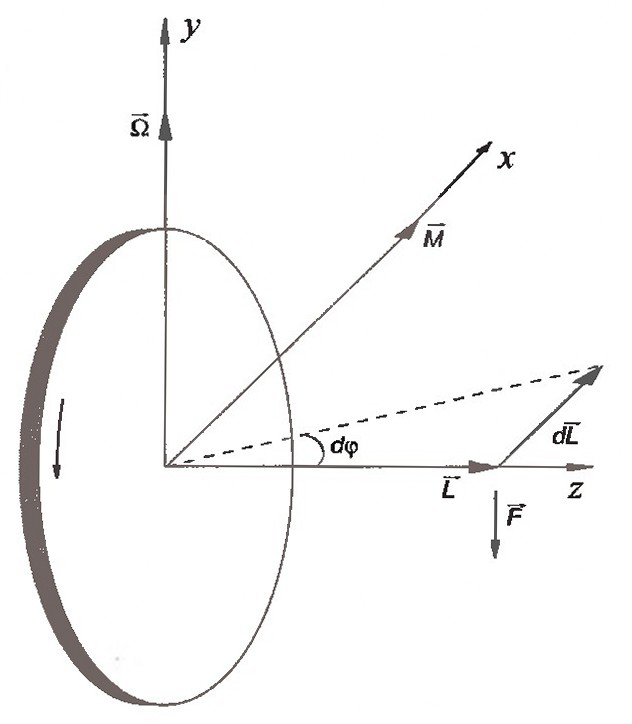
\includegraphics[width=\linewidth]{mahovic.jpg}}
		\caption{Маховик}
		\label{mah}
	\end{center}
\vspace{2cm}
\end{wrapfigure}
Тогда:
$$\abs{d \vec{L}} = Ld \varphi=L\Omega dt.$$
$$d \vec{L} = \vec{\Omega} \times \vec{L} dt,$$
$$\text{или}$$
$$\cfrac{d \vec{L}}{dt} = \vec{\Omega} \times \vec{L}.$$
В силу \eqref{2}:
\begin{equation}
\boxed{
\vec{M} = \vec{\Omega} \times \vec{L}}.
\label{6}
\end{equation}

Формула \eqref{6} справедлива только при условии \eqref{5} и отражает установившийся процесс. Она позволят определить момент сил $\vec{M}$, который необходимо приложить к маховику для того, чтобы вызвать прецессию маховика с угловой скоростью $\vec{\Omega}$.

Найдём угловую скорость прецессии гироскопа, к оси которого подвешен груз массой $m$. Сама же ось наклонена на угол $\alpha$ от вертикали:

\begin{center}
\vspace{-20pt}
\begin{equation}
\Omega = \cfrac{M}{I_z \omega_0 \sin \alpha}= \cfrac{mgl \sin \alpha}{I_z \omega_0 \sin \alpha} = \cfrac{mgl}{I_z \omega_0}\,,
\label{7}
\end{equation}
\end{center}
где $m$~--- масса груза, $g$~--- ускорение свободного падения, $l$~--- расстояние от центра масс гироскопа до точки крепления груза на оси гироскопа.

Теория и рисунки взяты из \cite{Gladun:PrakMech}~--- c. 160~--~162.
\textbf{\section{Экспериментальная установка}}
Экспериментальная установка для исследования прецессии уравновешенного гироскопа показана на рис. \ref{ris2}. Ротором гироскопа является ротор высокоскоростного электромотора M, питающегося током частотой 400 Гц. Кожух мотора сцеплен с кольцом Б. Мотор с кольцом Б может вращаться в~кольце А вокруг горизонтальной оси, которое может вращаться вокруг вертикальной оси. Ротор электромотора представляет массивный стальной цилиндр с прожилками меди, образующими <<беличье колесо>>. Рычаг С направлен по оси симметрии ротора. На рычаг подвешивают грузы Г. Подвешивая различные грузы, можно менять силу $F$, момент которой определяется расстоянием $l$ от точки подвеса до горизонтальной оси кольца А (до центра масс гироскопа).

Вследствие действия сил трения, ось гироскопа будет опускаться в~направлении действия груза, и появится вращение, значение угловой скорости которого есть $\Omega_{\text{опуск}}$. Вектор $\vec{\Omega}_{\text{опуск}}$ перпендикулярен плоскости рисунка и направлен от читателя.

Описание экспериментальной установки взято из \cite{Gladun:PrakMech}~--- c. 163~--~165.

\begin{figure}[h]
\vspace{60pt}
  \begin{center}
    \fbox{
    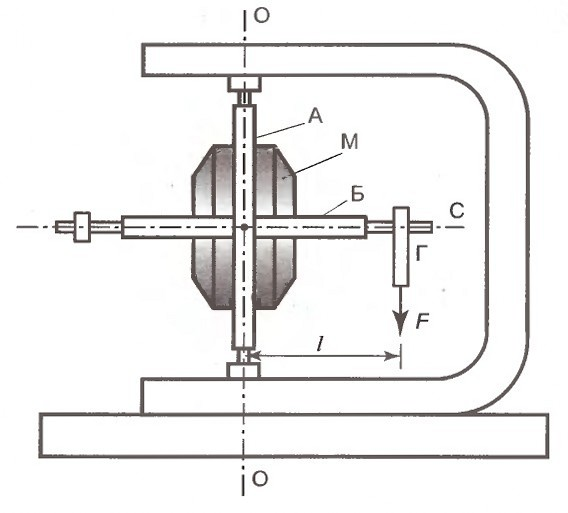
\includegraphics[width=0.7\textwidth]{ust.jpg}}
	\caption{Схема экспериментальной установки}
	\label{ris2}
  \end{center}
\end{figure}

\textbf{\section{Обработка результатов измерений}}
\subsection{Измерение значения $\omega_0$ гироскопа через значение $\Omega$ вынужденной прецессии}
\subsubsection{Определение величины $I_z \omega_0$}
Подвесим различные грузы на рычаг и измерим время, за которое он сделает полный оборот $N$ раз. Тогда  можно измерить $\Omega$ по формуле:
$$\Omega = 2 \pi \cfrac{N}{t}\,,$$
момент сил $M$:
$$M=mgl,$$
а также найдем стандартную ошибку $\sigma_{\Omega}$:
$$\sigma_{\Omega}=\sqrt{\cfrac{\sum \limits_{i=1}^3 (\Omega_i - \bar{\Omega})^2 \quad}{3-1}}=\sqrt{\cfrac{\sum \limits_{i=1}^3 (\Omega_i - \bar{\Omega})^2 \quad}{2}}.$$
Усредним результаты и занесём в~таблицу \ref{tab1}.
\begin{table}[h!]
\centering
\caption{ }
\label{tab1}
\setlength{\extrarowheight}{1mm}
\begin{tabular}{|c|c|c|c|c|}
\hline
$m$, кг & $\Omega$, $\text{с}^{-1}$ & $l$, м                 & $M$, Н$\cdot$м & $\sigma_{\Omega}$, $10^{-4}$ $\text{с}^{-1}$ \\ \hline
0.057   & 0.029              & \multirow{6}{*}{0.119} & 0.066           & 2.6                                            \\ \cline{1-2} \cline{4-5} 
0.093   & 0.048              &                        & 0.11            & 0.61                                           \\ \cline{1-2} \cline{4-5} 
0.142   & 0.073              &                        & 0.17            & 0.97                                           \\ \cline{1-2} \cline{4-5} 
0.179   & 0.093              &                        & 0.21            & 1.8                                            \\ \cline{1-2} \cline{4-5} 
0.274   & 0.14               &                        & 0.32            & 5.8                                            \\ \cline{1-2} \cline{4-5} 
0.342   & 0.18               &                        & 0.40            & 5.1                                            \\ \hline
\end{tabular}
\end{table}
\setlength{\extrarowheight}{0mm}

Нанесём на график экспериментальные точки $\Omega (M)$ и проведём по ним прямую методом наименьших квадратов (МНК, через начало координат, рис. \ref{graph}).
\begin{figure}[h!]
  \begin{center}
    \includegraphics[width=0.75\textwidth]{prec.eps}
    \caption{Зависимость угловой скорости прецессии $\Omega$ от приложенного момента сил тяжести $M$}
    \label{graph}
  \end{center}
\end{figure}
Тогда величина обратная тангенсу угла наклона прямой из \eqref{7} равна $I_z \omega_0$:
\begin{center}
$\cfrac{1}{\tan\varphi}=I_z \omega_0 = \cfrac{1}{0.444}$ $\cfrac{\text{кг} \cdot \text{м}^2}{\text{с}}=2.27\  \cfrac{\text{кг} \cdot \text{м}^2}{\text{с}}$.
\end{center}
Из МНК:
$$
\sigma_{\tan\varphi} = \cfrac{1}{\sqrt{n}} \sqrt{\cfrac{<\Omega^2>}{<M^2>}-\tan^2\varphi} = 0.012\  \cfrac{\text{с}}{\text{кг}\cdot \text{м}^2}.
$$
Найдём $\sigma_{I_z \omega_0}$ из формулы:
$$
\pogk{\tan \phi}=\pogk{I_z \omega_0} \Rightarrow \sigma_{I_z \omega_0} = 0.06\ \cfrac{\text{кг}\cdot\text{м}^2}{\text{с}}.
$$
Тогда получим, что:
\begin{equation}
    \fbox{
    $I_z \omega_0 = 2.27 \pm 0.06\ \cfrac{\text{кг}\cdot \text{м}^2}{\text{с}}$}.
	\label{8}
\end{equation}
\subsubsection{Измерение момента инерции ротора $I_z$}
Момент инерции ротора относительно оси симметрии измеряется по крутильным колебаниям точной копии ротора, подвешиваемой вдоль оси симметрии на жёсткой проволоке. Период крутильных колебаний $T_0$ зависит от момента инерции $I_z$ и модуля кручения проволоки $f$:
\begin{equation}
    T_0=2 \pi \sqrt{\cfrac{I_z}{f}}.
\end{equation}

Чтобы исключить $f$, вместо ротора гироскопа к той же проволоке подвешивают цилиндр правильной формы с известными размерами и массой, для которого легко можно вычислить момент инерции $I_{\text{ц}}$. Тогда получим выражение для определения момента инерции ротора гироскопа:
\begin{equation}
    I_z=I_\text{ц}\, \cfrac{T_0^2}{T_\text{ц}^2}\,,
    \label{10}
\end{equation}
где $T_\text{ц}$~--- период крутильных колебаний цилиндра.

Теория взята из \cite{Gladun:PrakMech}~--~c. 165.

Измерение периода крутильных колебаний проведём 3 раза и усредним значения. Для этого измерим время за которое совершается 10 крутильных колебаний и найдём периоды $T_0$ и $T_\text{ц}$. Также найдём стандартные ошибки  $\sigma_{T_0}$ и $\sigma_{T_\text{ц}}$. Получим:
$$T_0 = 8.42 \pm 0.03\  \text{с},\qquad T_\text{ц} = 10.612 \pm 0.012\  \text{c}.$$

С помощью штангенциркуля получим значение диаметра цилиндра $d=(7.90 \pm 0.01)\cdot 10^{-2}$ м.\\
Т.к. $I_\text{ц}= \frac{1}{2}\, m_\text{ц}R^2=\frac{1}{2}\, m_\text{ц} \left(\frac{d}{2} \right)^2=\frac{1}{8}\, m_\text{ц}d^2$, где $m_\text{ц}$ --- масса цилиндра, равная $m_\text{ц}=(1618.9 \pm 0.5)\cdot 10^{-3}$ кг. Найдём стандартную ошибку $\sigma_{I_\text{ц}}$ по формуле:
$$
\pogk{I_\text{ц}}=\pogk{m_\text{ц}}+4\pogk{d}.
$$
Подставив, получим:
$$
I_\text{ц}=(1.263 \pm 0.003) \cdot 10^{-3}\  \text{кг} \cdot \text{м}^2.
$$
У нас есть все данные, чтобы получить $I_z$. Найдём стандартную ошибку $\sigma_{I_z}$ по формуле:
$$
\pogk{I_z}=\pogk{I_\text{ц}}+4\pogk{T_0}+4\pogk{T_\text{ц}}.
$$
Подставив полученные значения в~формулу \eqref{10}, получим:
\begin{center}
\vspace{-20pt}
\begin{equation}
\fbox{
$I_z=(8.16 \pm 0.06)\cdot 10^{-4}\  \text{кг} \cdot \text{м}^2$}.
\end{equation}
\end{center}

\subsubsection{Измерение значения $\omega_0$}
Теперь найдём $\omega_0$ из \eqref{8}, разделив значение $I_z \omega_0$ на значение $I_z$. Стандартную ошибку $\sigma_{\omega_0}$ получим по формуле:
$$
\pogk{\omega_0}=\pogk{I_z\omega_0}+\pogk{I_z}.
$$
Подставив значения, получим:
\begin{equation}
\fbox{
$\omega_0 = (2.82 \pm 0.08) \cdot 10^3\  \text{с}^{-1}$}.
\end{equation}
Видно, что $\omega_0 \gg \Omega$.
\subsection{Измерение значения $\omega_0$ гироскопа с помощью осциллографа}
Скорость вращения ротора гироскопа можно определить и не прибегая к исследованию прецессии. У используемых в~работе гироскопов статор имеет две обмотки, необходимые для быстрой раскрутки гироскопа. В данной работе одну обмотку используют для раскрутки гироскопа, а вторую~--- для измерения числа оборотов ротора. Ротор электромотора всегда немного намагничен. Вращаясь, он наводит во второй обмотке переменную ЭДС индукции, частота которой равна частоте вращения ротора. Частоту этой ЭДС можно измерить по фигурам Лиссажу, получаемым на экране осциллографа, если на один вход подать исследуемую ЭДС, а на другой~--- переменной напряжение с хорошо прокалиброванного генератора. При совпадении частот на экране получаем эллипс.

В данном эксперименте была получена частота $\nu = 439.0 \pm 0.5$ Гц. Тогда 
$$
\omega_{0_{\text{осц}}} =2 \pi \nu, \qquad \pogk{\omega_{0_{\text{осц}}}}=\pogk{\nu}.
$$
Подставив, получим:
\begin{equation}
    \fbox{
    $\omega_{0_{\text{осц}}}=2 \pi \nu = (2.758 \pm 0.003) \cdot 10^3\  \text{с}^{-1}$}.
\end{equation}

\subsection{Сравнение $\omega_0$ и $\omega_{0_{\text{осц}}}$}
Рассчитаем, насколько отличаются значения $\omega_0$, полученные разными способами:
$$
\delta=\cfrac{\abs{\omega_0-\omega_{0_{\text{осц}}}}}{\omega_{0_{\text{осц}}}} \cdot 100\, \% \simeq 2.2 \,\%.
$$

Видим, что значения $\omega_0$, полученные разными способами, достаточно близки друг к другу. 

\subsection{Расчёт значения $\Omega_{\text{опуск}}$}
С помощью линейки измерим высоту подъёма рычага. Повесим на него груз и через некоторое время снова измерим высоту подъёма рычага. Т.к. действуют силы трения, высота подъёма уменьшилась. В данном эксперименте это изменение равно $\Delta H = 0.008$ м, причём рычаг опустился за время $t_{\text{опуск}} = 170.36 $ с. Т.к. угол малый, считаем, что 
$$
\cfrac{\Delta H}{l_1}=\tan \alpha_{\text{опуск}} \approx \alpha_{\text{опуск}},
$$
где $\alpha_{\text{опуск}}$~--- угол, на который опустился рычаг, $l_1$ - полная длина рычага, равная $l_1=0.123$ м. 
Таким образом:
$$\alpha_{\text{опуск}} = \cfrac{\Delta H}{l_1} = 0.065\  \text{рад}.$$
Тогда найдём значение $\Omega_{\text{опуск}}$:
$$\Omega_{\text{опуск}} = \cfrac{\alpha_{\text{опуск}}}{t_{\text{опуск}}} \approx 3.8 \cdot 10^{-4}\  \text{с}^{-1}.$$
В силу \eqref{6}:
\begin{equation}
    \fbox{
    $M_{трения}= \Omega_{\text{опуск}} I_z \omega_0 \approx 0.87 \cdot 10^{-3} \sim 10^{-3}\,\text{Н} \cdot \text{м}$}.
\end{equation}
Видно, что момент сил трения мал, однако этого достаточно, чтобы рычаг гироскопа поворачивался в~сторону линии действия силы тяжести груза. 

\section{Заключение}
В данной работе мы наблюдали вынужденную прецессию гироскопа.

Определив угловую скорость прецессии $\Omega$, мы нашли значение угловой скорости вращения ротора гироскопа $\omega_0 = (2.82 \pm 0.08) \cdot 10^3\ \text{с}^{-1}$, которая почти совпадает (отличие на $2.2\, \%$)  со значением $\omega_{0_{\text{осц}}} = (2.758 \pm 0.003) \cdot 10^3\ \text{с}^{-1}$, измеренным с помощью осциллографа.

Также мы по порядку величины определили момент сил трения: $M_{\text{трения}} \sim 10^{-3}\ \text{Н} \cdot \text{м}$.


\bibliography{mybibliography}
\bibliographystyle{gost705}


























\end{document}
